\documentclass{article}

\usepackage{graphicx}

\title{Oscillators}
\author{Anderson Hsieh}
\date{July 18, 2026}

\begin{document}

\maketitle

\section{Questions Answered}
\begin{enumerate}
    \item Why do we use transient + FFT when simulating and analyzing oscillators in SPICE, instead of AC analysis frequency sweep?\\
    Becuse AC analysis assumes a DC operating point and runs small signal analysis based on that. When a oscillator is oscillating it's usually a large signal thing, thus there is no stable DC operating point. It's just not valid.
    \item Octave vs Matlab, what can they do that other things can't?\\
    it can be used to evaluate Lapalce domain transfer function, obtaining the frequency characteristics\\
    \begin{verbatim}
        f = logspace(3, 10, 10000);  % Hz
        w = 2*pi*f;                   % rad/s
        
        response = squeeze(freqresp(H, w));
        
        semilogx(f, 20*log10(abs(response)));
        grid on;
        xlabel("Frequency (Hz)");
        ylabel("Magnitude (dB)");

    \end{verbatim}
\end{enumerate}

\section{Questions To be Answered}
    \begin{enumerate}
        \item Figure out differential inverter for differential ring oscillator, fully understand the voltage swingrange of a single diff inverter.
        \item use Octave, write a transfer function of a filter, evaluate the filter shape, understand poles and zeros
        \item realize the filter designed in Octave with circuit elements and filter the ring oscillator output. 
    \end{enumerate}
\section{Some Picture}
    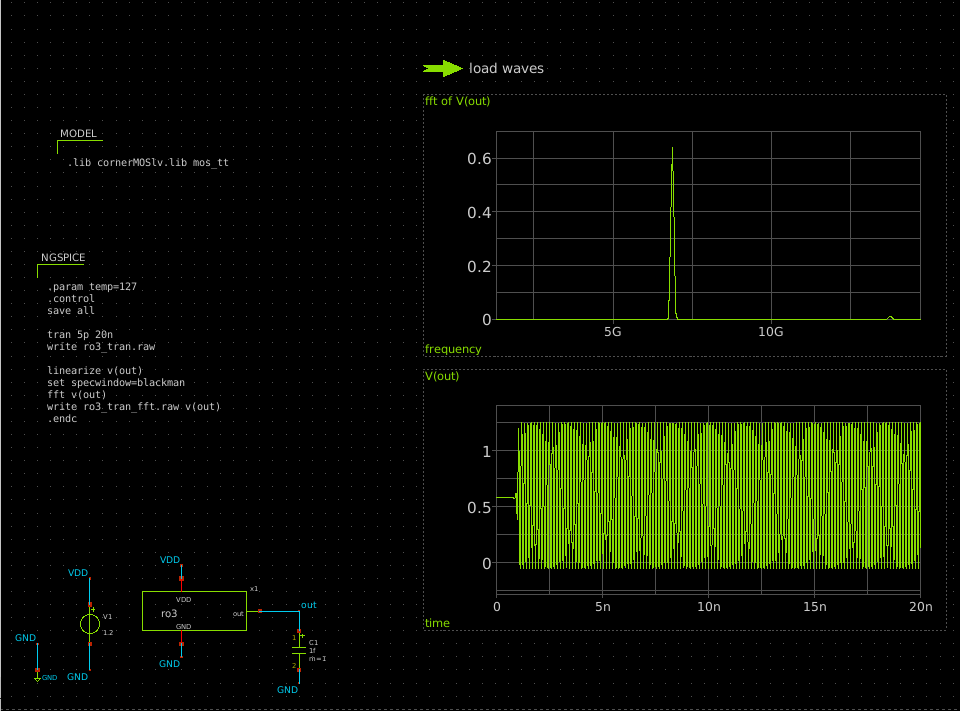
\includegraphics[width=\textwidth]{images/ro3_tb.png}
    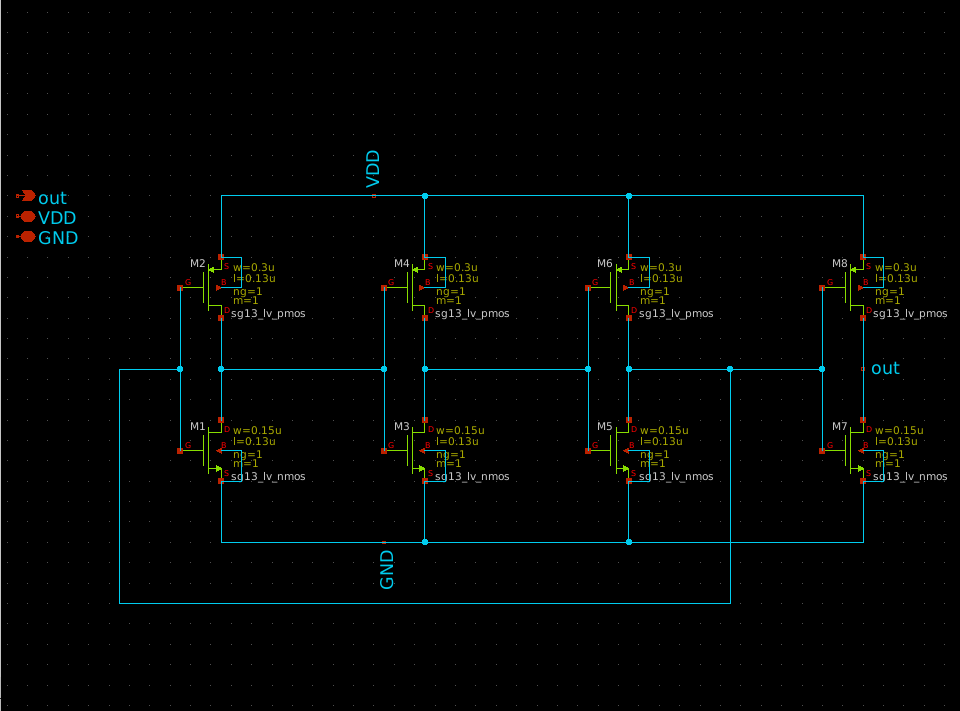
\includegraphics[width=\textwidth]{images/ro3.png}

\end{document}
